\section{Integrals}

The term "\keyword{integral}" encompasses several distinct concepts in mathematics. Its most prevalent meaning relates to the fundamental concept in calculus, where it involves the process of summing infinitesimally small components to determine the content of a continuous region. In calculus, an integral is a fundamental mathematical concept that can be interpreted as measuring area or extending the notion of area to more complex shapes. Alongside derivatives, integrals are the cornerstone of calculus. They are also referred to as \keyword{antiderivatives} or \keyword{primitives}. The act of evaluating an integral is known as integration (a term sometimes replaced by the more historical word "quadrature"). When an integral is approximated numerically, it is called numerical integration.

\begin{defn}[The Antiderivative]{1}
A function $F$ is called an \keyword{antiderivative} of a function $f$ on an interval $I$ if $\frac{d}{dx}F(x)=f(x)$ for all $x\in I$.
\end{defn}

\begin{figure}
  \centering
  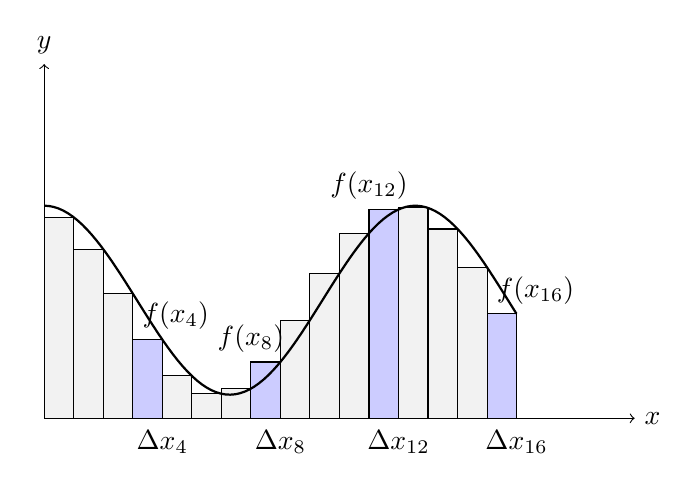
\begin{tikzpicture}[scale=1.5]
  % Define the function
  \def\f(#1){0.8*cos(deg(2*#1)) + 1}
  
  % Draw the x-axis
  \draw[->] (0,0) -- (5,0) node[right] {$x$};
  % Draw the y-axis
  \draw[->] (0,0) -- (0,3) node[above] {$y$};
  
  
  % Draw the rectangles for the Riemann sum
  \draw[fill=gray!10] (0, 0) rectangle (.25, {\f(.25)});
  \draw[fill=gray!10] (.25, 0) rectangle (.5, {\f(.5)});
  \draw[fill=gray!10] (.5, 0) rectangle (.75, {\f(.75)});
  \draw[fill=blue!20] (0.75, 0) rectangle (1, {\f(1)});
  \draw[fill=gray!10] (1, 0) rectangle (1.25, {\f(1.25)});
  \draw[fill=gray!10] (1.25, 0) rectangle (1.5, {\f(1.5)});
  \draw[fill=gray!10] (1.5, 0) rectangle (1.75, {\f(1.75)});
  \draw[fill=blue!20] (1.75, 0) rectangle (2, {\f(2)});
  \draw[fill=gray!10] (2, 0) rectangle (2.25, {\f(2.25)});
  \draw[fill=gray!10] (2.25, 0) rectangle (2.5, {\f(2.5)});
  \draw[fill=gray!10] (2.5, 0) rectangle (2.75, {\f(2.75)});
  \draw[fill=blue!20] (2.75, 0) rectangle (3, {\f(3)});
  \draw[fill=gray!10] (3, 0) rectangle (3.25, {\f(3.25)});
  \draw[fill=gray!10] (3.25, 0) rectangle (3.5, {\f(3.5)});
  \draw[fill=gray!10] (3.5, 0) rectangle (3.75, {\f(3.75)});
  \draw[fill=blue!20] (3.75, 0) rectangle (4, {\f(4)});
  
  % Draw the curve
  \draw[thick, domain=0:4, samples=100] plot (\x, {\f(\x)});
  
  % Draw the labels for f(xi)
  \draw (0.75, {\f(1)}) node[above right] {$f(x_{4})$};
  \draw (1.75, {\f(2)}) node[above] {$f(x_{8})$};
  \draw (2.75, {\f(3)}) node[above] {$f(x_{12})$};
  \draw (3.75, {\f(4)}) node[above right] {$f(x_{16})$};
  
  % Draw the arrows for delta x
  
  \draw (1, -0.2) node {$\Delta x_{4}$};
  \draw (2, -0.2) node {$\Delta x_{8}$};
  \draw (3, -0.2) node {$\Delta x_{12}$};
  \draw (4, -0.2) node {$\Delta x_{16}$};
  \end{tikzpicture}
  \caption{A visualization of the Riemann Sums. The partition width is denoted by $\Delta x_i$ and the height of the partitions is $f(x_i)$.}
  \label{fig:Riemann Sum visualization}
\end{figure}

\begin{defn}[Riemann Sum\label{defn:Riemann Sum]{1}
Let $f$ be defined on the closed interval $[a,b]$, and let $\Delta$ be a partition of $[a,b]$ given by $a=x_0 < x_1 < \cdots < x_{n-1} < x_n = b$, where $\Delta x_i$ is the width of the $i$th sub-interval. If $c_i \in [x_{i-1},x_i]$, then the sum $\sum_{i=1}^{n}f(c_i)\Delta x_i$ is called a Riemann sum of $f$ for the partition $\Delta$.
\end{defn}

The largest width among the subintervals within a partition $\Delta$ is known as the partition's norm, represented by $||\Delta||$. If all subintervals have equal width, the partition is called regular, and its norm is denoted by $||\Delta|| = \Delta x = \frac{b-a}{n}$. The integral can be defined in the limit as this partition's norm approaches zero $||\Delta|| \to 0$. Therefore, there exists some $L\in\mathbf{R}$ such that for each $\epsilon > 0$, there exists a $\delta > 0$ so that for all partitions with $||\Delta|| < \delta$, we have

\begin{align}
\lim_{||\Delta|| \to 0}\sum_{i=1}^{n}f(c_i)\Delta x_i = L \implies \bigg|L-\sum_{i=1}^{n}f(c_i)\Delta x_i\bigg| < \epsilon
\end{align}

This then give the definition of the definite integral.

\begin{defn}[The Definite Integral\label{defn:The Definite Integral}]{1}
IF $f$ is defined on the closed interval $I=[a,b]$ and the limit of the Riemann sums over partitions $\Delta$ exists, then $f$ is said to be integrable on $I$ and the limit is denoted by the definite integral of $f$ from $a$ to $b$. 
\begin{align}
\lim_{||\Delta|| \to 0}\sum_{i=1}^{n}f(c_i)\Delta x_i = \int_a^b f(x)dx
\end{align}
\end{defn}

%\begin{theo}[The Fundamental Theorem Of Calculus]{1}
%Suppose that $f(x)$ is continuous on the interval [a,b]. If $F(x)$ is any antiderivative of $f(x)$, then $\int_a^b f(x) dx = F(b)-F(a)$. Given $F(x) = \int_a^b f(x) dx$, then $\frac{d}{dx}F(x) = f(x)$.
%\end{theo}
